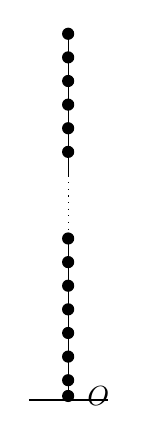
\begin{tikzpicture}
  % vertical string with beads (point masses), dotted gap in the middle
  \draw (0,4.8) -- (0,3.0);
  \draw[dotted] (0,3.0) -- (0,2.2);
  \draw (0,2.2) -- (0,0.2);
  % upper beads
  \foreach \y in {4.8,4.5,4.2,3.9,3.6,3.3} { \fill (0,\y) circle (2.2pt); }
  % lower beads
  \foreach \y in {2.2,1.9,1.6,1.3,1.0,0.7,0.4} { \fill (0,\y) circle (2.2pt); }
  % ground / support at O
  \draw[thick] (-0.5,0.15) -- (0.5,0.15);
  \fill (0,0.2) circle (2.2pt);
  \node[right] at (0.12,0.2) {$O$};
\end{tikzpicture}
